% Drop-in Supporting Information section for the CRPS ensemble U-Net paper.
% Companion assets live in this folder (figures/si/), including the
% ensemble-size 3×2 panel (suggested Fig.~S1).
%
% Main-text explainability figure: ../main/13_explainability_main.pdf
%   \label{fig:explainability}
%
% Suggested SI numbering when including ensemble-size sensitivity first:
%   Fig.~S1  -- ensemble-size rank hist + SSR (M=4,8,16)
%   Fig.~S2  -- expanded bottleneck PCA colorings
%   Fig.~S3  -- additional integrated-gradient cases
%   Fig.~S4  -- IG attribution by predictor group
%   Table~S1 -- full permutation-importance numbers

\section{Additional Model Explainability Diagnostics}
\label{sec:si_explainability}

The main text (Fig.~\ref{fig:explainability}) summarizes the strongest
explainability diagnostics for the CRPS ensemble U-Net: bottleneck PCA
colored by $P(S>\tau^*)$ and $N_{\mathrm{amb}}$, predictor-group permutation
effects on almost-fair CRPS and Brier skill, and one integrated-gradient (IG)
spatial example. This section provides the complementary panels and the full
numerical tables.

Unless noted otherwise, analyses use the frozen ASCAT-A validation split with
fixed latent-noise seeds, $\tau^*=1.2\times10^{-4}$, and the same 19 ASCAT
predictor groups as in the main text
(smooth wind context; rain/retrieval QC; $N_{\mathrm{amb}}$; ambiguity winds/SOS).

%--------------------------------------------------------------------------
\subsection{Bottleneck Representation}
\label{sec:si_bottleneck}

Figure~\ref{fig:si-explain-pca} expands the bottleneck PCA embedding with
additional physical covariates (target Sobel field $S$, smoothed wind-gradient
magnitude, smoothed wind speed, and rain flag). Together with
Fig.~\ref{fig:explainability}a,b these colorings show that the latent
representation organizes both cold-pool-related magnitude and retrieval /
QC state, rather than collapsing onto a single input channel.

\begin{figure}[t]
\centering
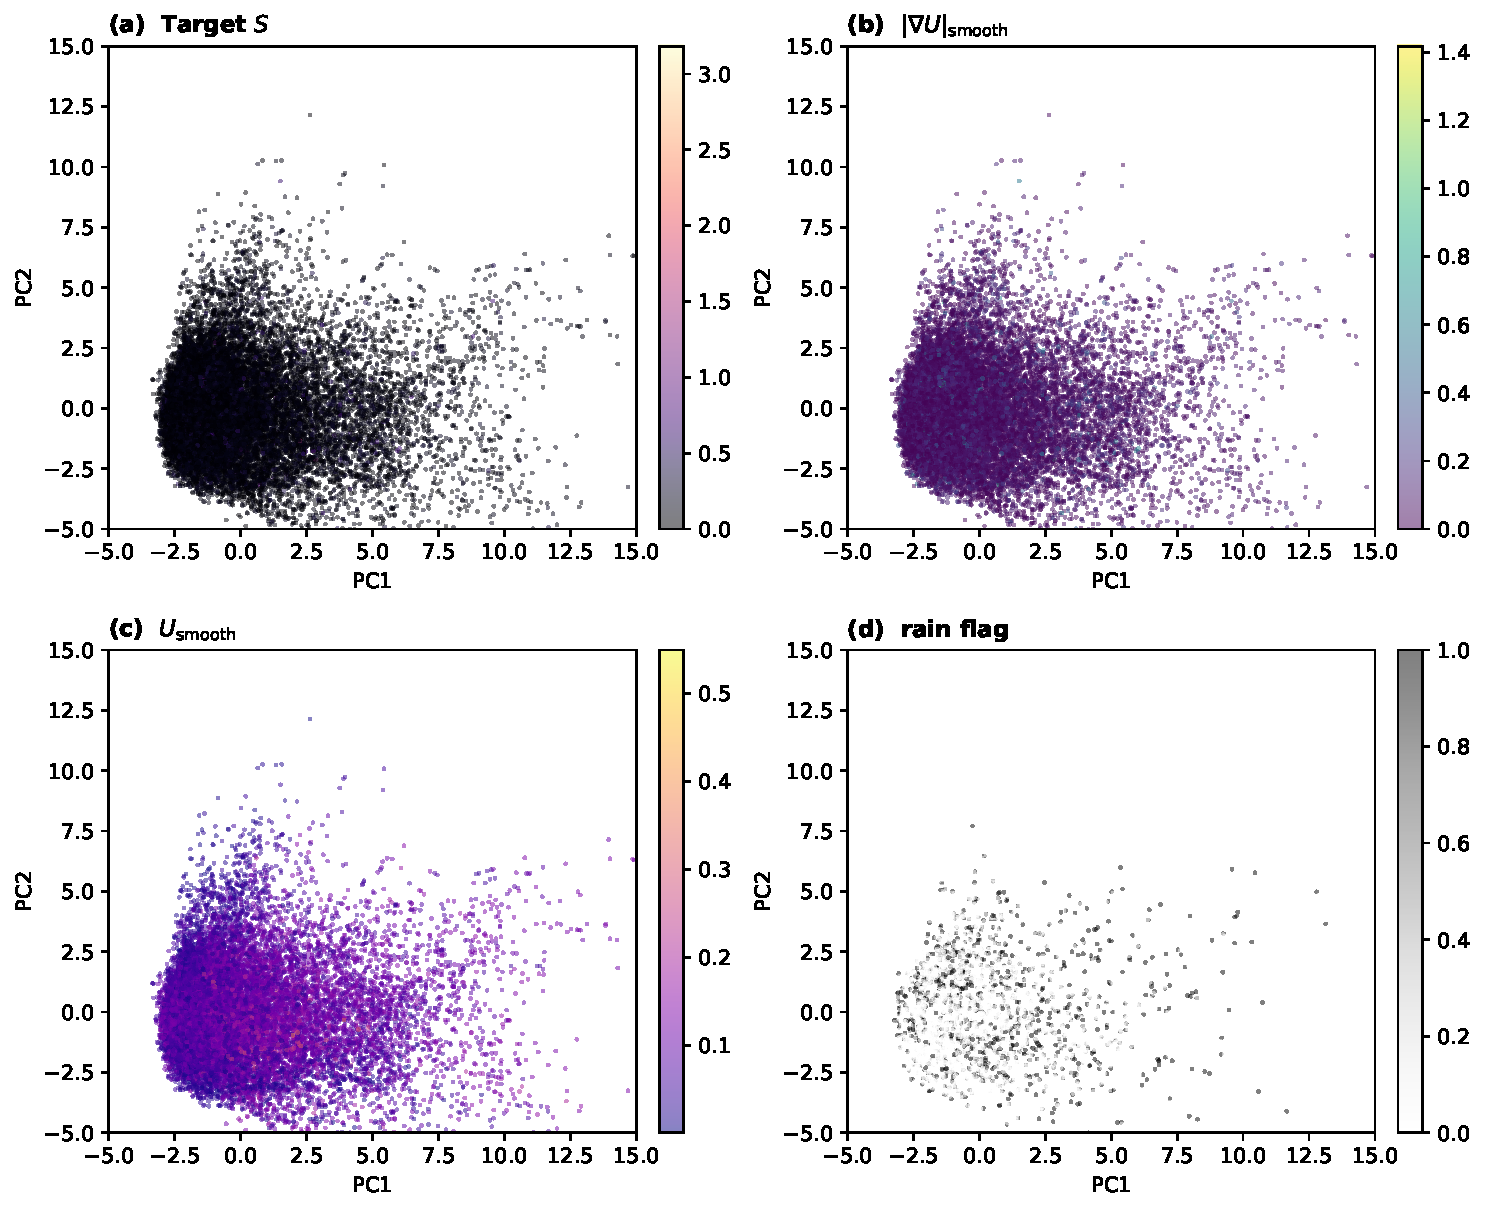
\includegraphics[width=\textwidth]{SI_explain_pca_extra.pdf}
\caption{Expanded bottleneck PCA diagnostics (Supporting Information).
Same embedding as Fig.~\ref{fig:explainability}a,b (PC1--PC2;
axis limits $[-5,15]$), colored by (a)~target $S$,
(b)~$|\nabla U|_{\mathrm{smooth}}$, (c)~$U_{\mathrm{smooth}}$, and
(d)~rain flag. Main-text panels emphasize $P(S>\tau^*)$ and
$N_{\mathrm{amb}}$.}
\label{fig:si-explain-pca}
\end{figure}

%--------------------------------------------------------------------------
\subsection{Integrated-Gradient Attribution}
\label{sec:si_ig}

Figure~\ref{fig:si-explain-ig-cases} shows IG attribution for three
representative validation orbits (including the main-text example), with
left and right swath halves stitched along the cross-track axis. For each
orbit we display soft $P(S>\tau^*)$, $|\mathrm{IG}|$ summed over all ASCAT
channels, the $|\nabla U|_{\mathrm{smooth}}$ input for reference, and
$|\mathrm{IG}|$ restricted to the ambiguity winds/SOS group. Attributions
concentrate on coherent gust-front-scale streaks rather than isolated
retrieval artifacts.

\begin{figure}[t]
\centering
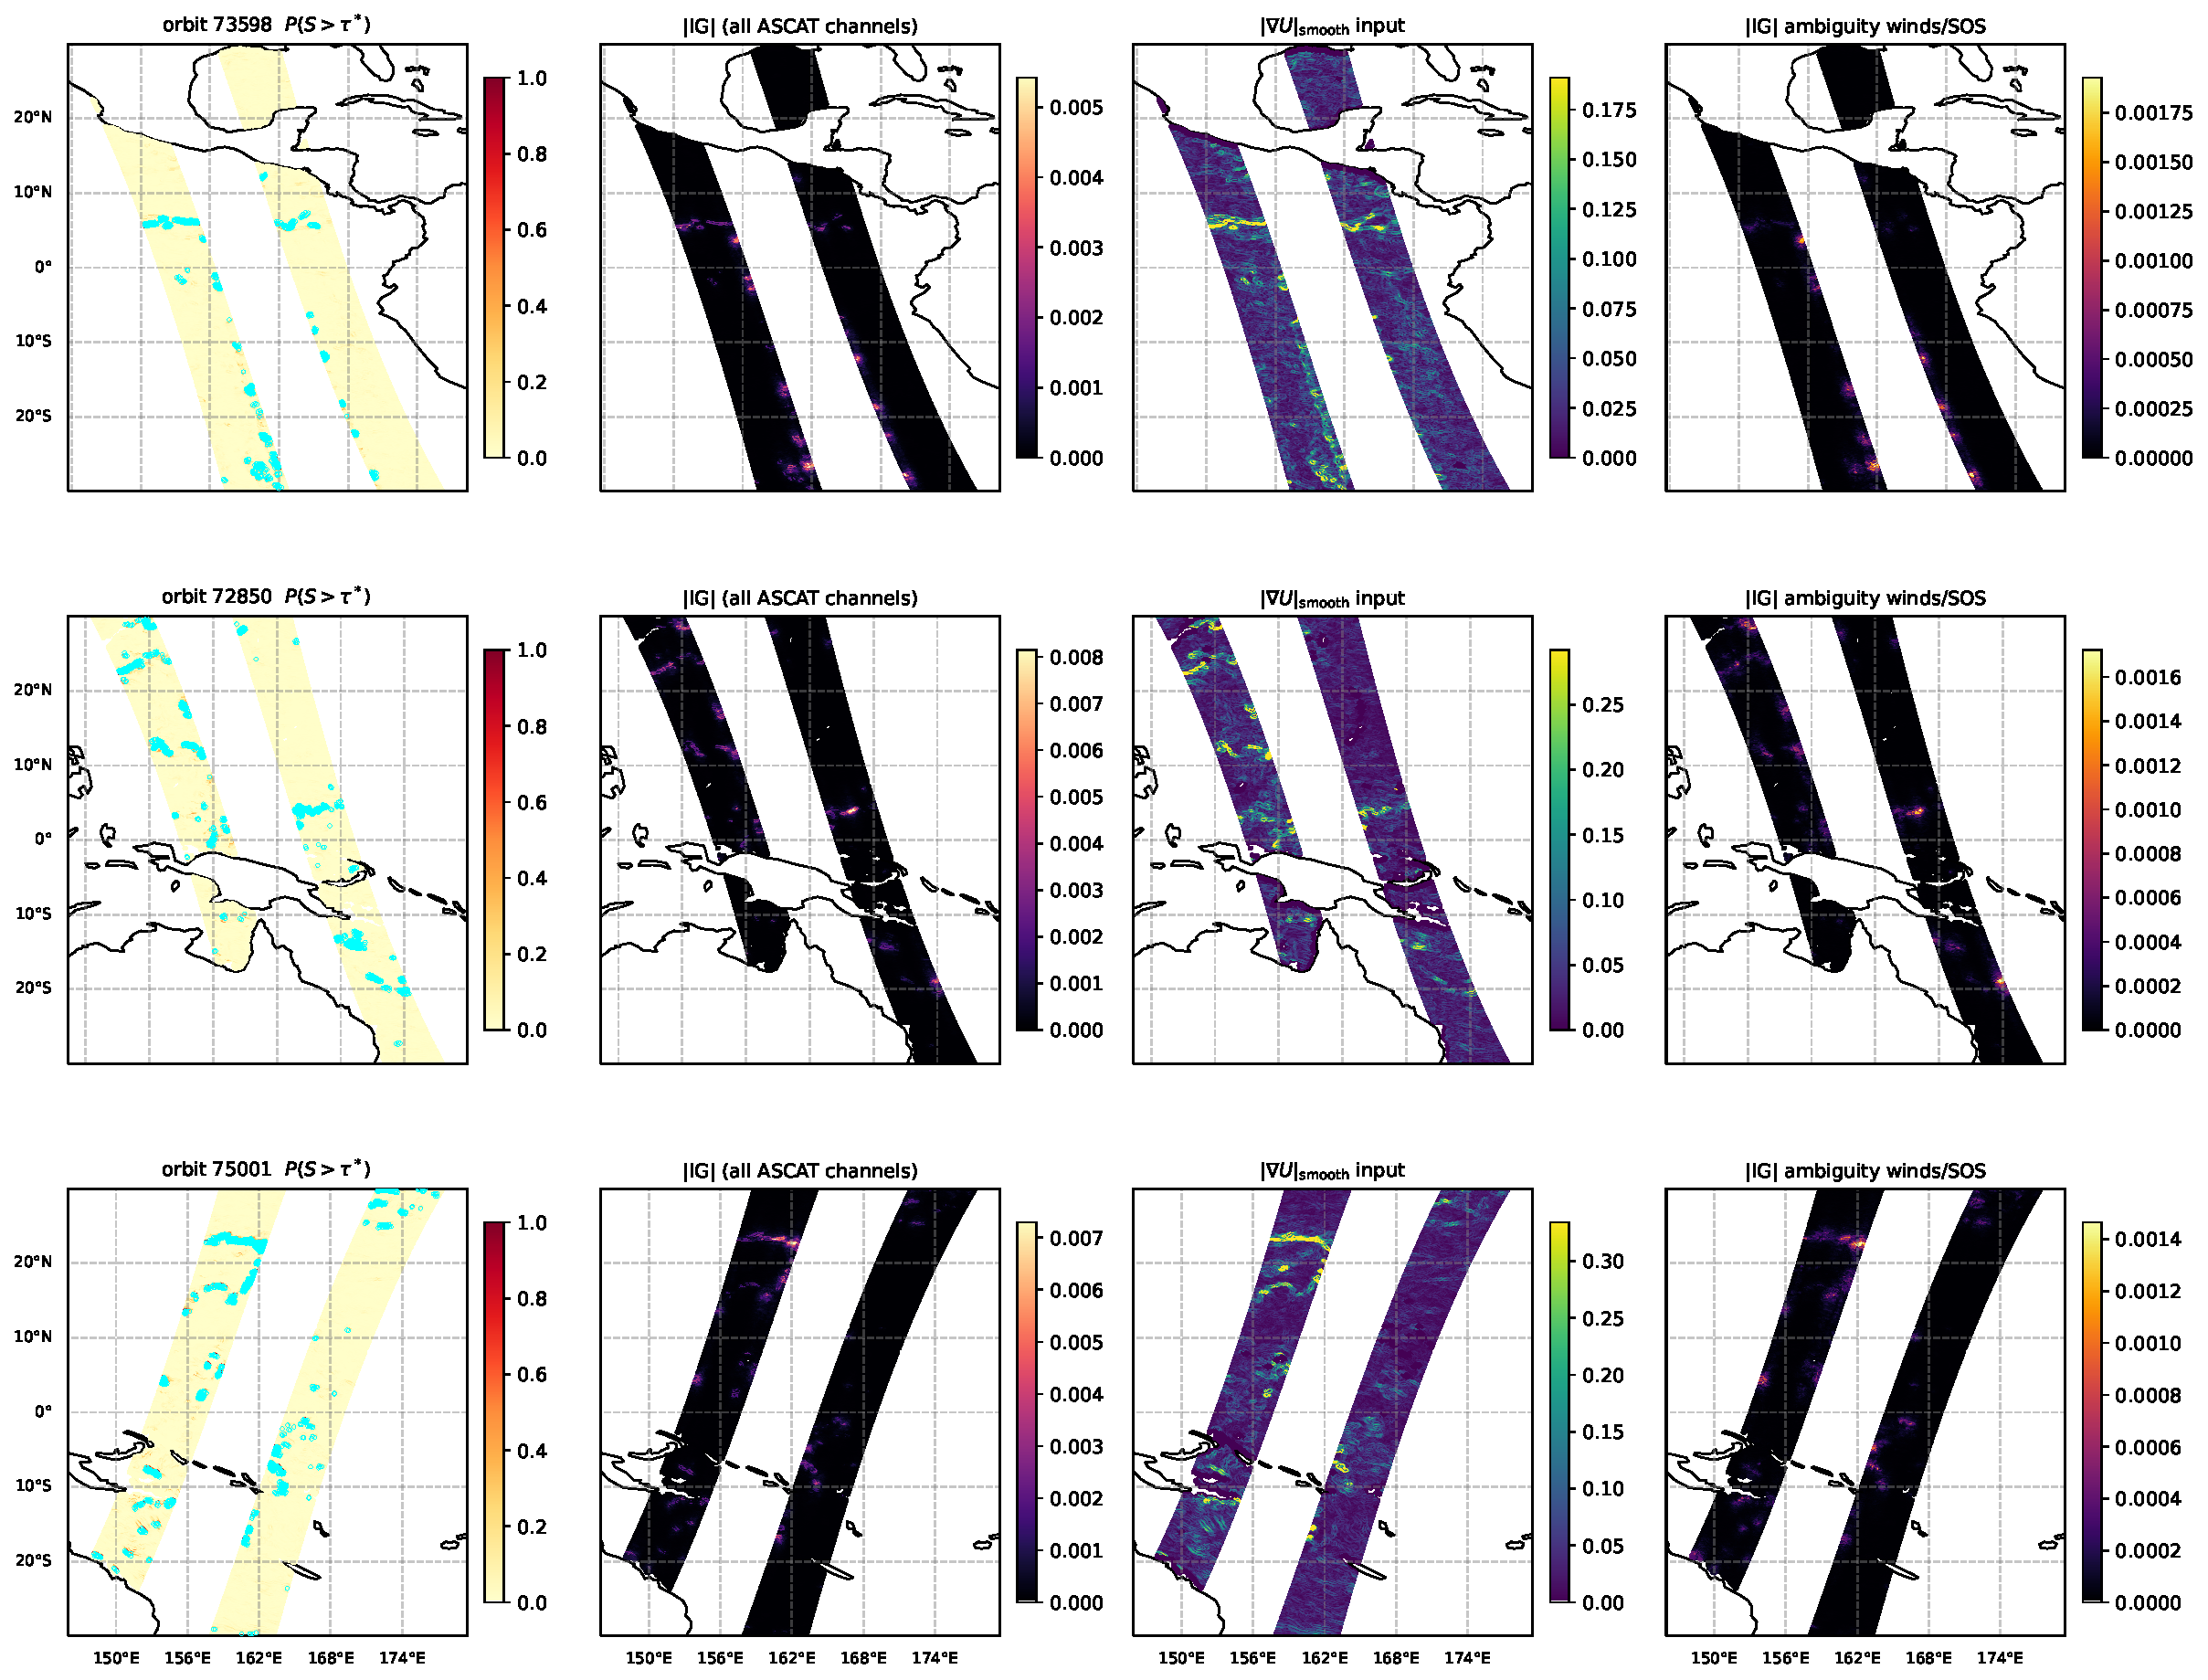
\includegraphics[width=\textwidth]{SI_explain_ig_cases.pdf}
\caption{Additional integrated-gradient examples (Supporting Information).
Rows: orbits 73598, 72850, and 75001. Columns: $P(S>\tau^*)$,
$|\mathrm{IG}|$ over all ASCAT channels, $|\nabla U|_{\mathrm{smooth}}$ input,
and $|\mathrm{IG}|$ from ambiguity winds/SOS. Each panel shows the
left$|$right swath (horizontal divider). Cyan contours mark the high-$P$
ROI used for attribution.}
\label{fig:si-explain-ig-cases}
\end{figure}

%--------------------------------------------------------------------------
\subsection{Attribution by Predictor Group}
\label{sec:si_ig_groups}

Figure~\ref{fig:si-explain-ig-share} summarizes the fraction of ROI
$|\mathrm{IG}|$ assigned to each predictor group for every orbit and swath
half. Smooth wind context typically accounts for $\sim$60--70\% of the
attribution mass, with ambiguity winds/SOS contributing a clear minority
share ($\sim$11--16\%), consistent with the main-text spatial example.

\begin{figure}[t]
\centering
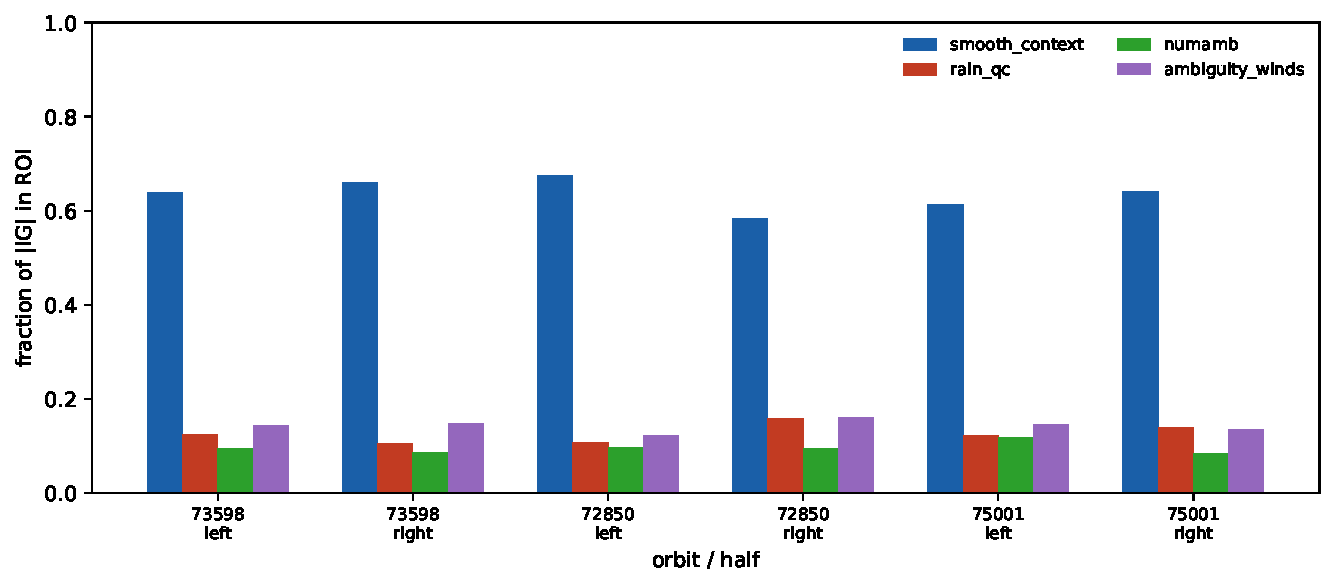
\includegraphics[width=0.9\textwidth]{SI_explain_ig_group_share.pdf}
\caption{Integrated-gradient attribution by predictor group (Supporting
Information). Bars show the fraction of ROI $|\mathrm{IG}|$ attributed to
smooth wind context, rain/retrieval QC, $N_{\mathrm{amb}}$, and ambiguity
winds/SOS, for each orbit and left/right swath half.}
\label{fig:si-explain-ig-share}
\end{figure}

Table~\ref{tab:si_ig_group_share} lists the corresponding numerical
fractions.

\begin{table}[htbp]
\centering
\caption{Fraction of ROI $|\mathrm{IG}|$ by predictor group for the three
integrated-gradient case orbits (left and right swath halves).}
\label{tab:si_ig_group_share}
\begin{tabular}{llcccc}
\toprule
Orbit & Half & Smooth context & Rain/QC & $N_{\mathrm{amb}}$ & Ambiguity winds/SOS \\
\midrule
73598 & left  & 0.638 & 0.124 & 0.094 & 0.144 \\
73598 & right & 0.661 & 0.105 & 0.087 & 0.148 \\
72010 & left  & 0.686 & 0.116 & 0.083 & 0.114 \\
72010 & right & 0.642 & 0.111 & 0.088 & 0.158 \\
75001 & left  & 0.614 & 0.121 & 0.118 & 0.147 \\
75001 & right & 0.641 & 0.139 & 0.084 & 0.136 \\
\bottomrule
\end{tabular}
\end{table}

%--------------------------------------------------------------------------
\subsection{Predictor-Group Permutation Importance}
\label{sec:si_permutation}

The main-text bar chart (Fig.~\ref{fig:explainability}c) summarizes
along-track permutation of predictor groups. Table~\ref{tab:si_permutation}
gives the full numerical results: change in held-out almost-fair CRPS and
Brier score at $\tau^*$ relative to the unperturbed baseline (positive
values indicate degradation). Smooth wind context dominates continuous-field
afCRPS degradation, whereas $N_{\mathrm{amb}}$ and ambiguity winds/SOS
contribute most to exceedance Brier degradation.

% Auto-generated from SI_tab_permutation.csv — digits copied verbatim from CSV.
% Source: evaluation/explainability/crps/13_predictor_group_permutation.csv
\begin{table}[htbp]
\centering
\caption{Predictor-group permutation importance on the ASCAT-A validation
sample used for Fig.~\ref{fig:explainability}c ($n=40$ swath halves;
fixed latent seeds). Values are changes relative to the unperturbed
baseline; positive values indicate degradation in predictive performance.
Baseline afCRPS $=0.006025998127581029$; baseline Brier $=0.00485630002767306$.
All digits are copied from the machine-readable table
\texttt{SI\_tab\_permutation.csv}.}
\label{tab:si_permutation}
\begin{tabular}{lcc}
\toprule
Predictor group & $\Delta$afCRPS & $\Delta$Brier \\
\midrule
Smooth wind context ($U$, $|\nabla U|$) & $+0.03815644820608599$ & $+0.00966971874226391$ \\
Rain / retrieval QC & $+0.03196630530970533$ & $+0.008596426527983998$ \\
$N_{\mathrm{amb}}$ & $+0.01890569752066945$ & $+0.015046991054192223$ \\
Ambiguity winds / SOS & $+0.015380771553790654$ & $+0.013772426016890625$ \\
\bottomrule
\end{tabular}
\end{table}
